\documentclass[12pt]{article}
\usepackage{graphicx}
\graphicspath{ {./images/} }

\title{Jelgenerátor, négyszög és háromszög jel generálása}
\author{Mészáros Adél}

\begin{document}
  \maketitle
  \newpage

  \section{Terv specifikálása}
   
  \paragraph{} 
    A laborgyakorlat célja egy olyan áramkör megvalósítása FPGA segítségével,
    amely képes háromszög és négyszög jelek generálására. A felhasználó kiválaszthatja,
    hogy milyen tipusú jelet szeretne generálni és állithatja annak amplitudóját és frekvenciáját.

    \paragraph{}
    A hardvert két fő komponens alkotja: 
    
    \begin{enumerate}
      \item Jelgenerátor
      \item Digitál-analóg konverter
    \end{enumerate}

    \section{Digitál-analóg konverter}
    Az AD5302/AD5312/AD5322 tipusú digitál-analóg tipusó konvertert fogom használni.

    \begin{figure}[h]
      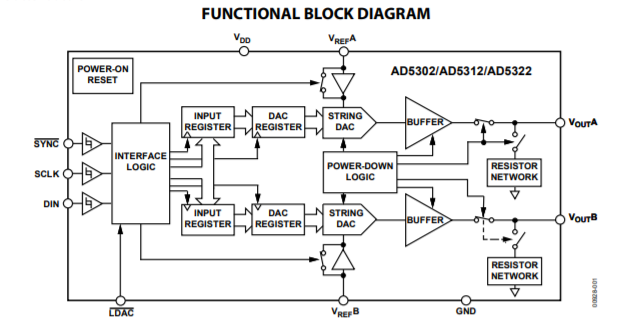
\includegraphics{dac_kapcs}
      \centering
    \end{figure}

    \begin{figure}[h]
      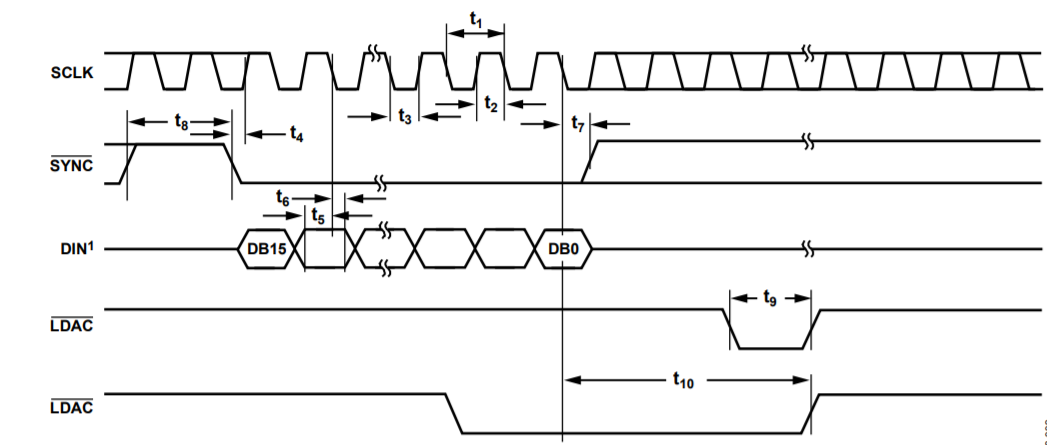
\includegraphics{dac_jelek}
      \centering  
    \end{figure}
    
    \begin{itemize}
      \item \textbf{LDAC} \linebreak
            \quad 0 - kimenet frissítése \linebreak
            \quad 1 - kimeneti érték változatlan
      \item \textbf{SYNC} \linebreak
            \quad 0 - bemeneti regiszter feltöltésének kezdése \linebreak
            \quad 1 - ha a bemeneti regiszter nem volt feltöltve, a feltöltés megszakad
      \item \textbf{SCLK} \linebreak
            \quad A bemeneti regiszter feltöltését ütemező órajel. Minden lemenő élre újabb bit töltődik be.
            A 16. bit betöltése után írhatóvá válik.  
      \item \textbf{DIN} \linebreak
            \quad A regiszter betöltött bit értéke
      \item \textbf{PDo, PD1} \linebreak
            \quad Power-down mode, ha mindkettő '0', normál üzemmód, máskülönben energiatakarékos üzemmód.
      \item \textbf{BUF} \linebreak
            \quad a reference buffer, ha '0', az ADC, 0-tól Vref-ig üzemel, ha '1' az ADC 1-től Vref-ig üzemel.
      \item \textbf{A/B} \linebreak
            \quad 0 - az A kimenetet (használja) updateolja \linebreak
            \quad 1 - a B kimenetet (használja) updateolja
    \end{itemize}
    
    \paragraph{Időzítések}
    \begin{itemize}
      \begin{itemize}
        \item \textbf{SCLK} periódus, minimum 33 ns
        \item \textbf{DIN} minimum 5 ns-el az órajel lemenő éle előtt és az órajel lemenő éle után
        \item \textbf{SYNC} minimum 100 ns 'high', az olvasások között. Az órajel felmenő éle előtt (vagy azzal egyszerre) kell lehúzni, hogy elkedjük az olvasást
      \end{itemize}
      
    \end{itemize}
    \begin{itemize}
      \item \textbf{SCLK} periódus, minimum 33 ms
    \end{itemize}

\end{document}
